\newpage
\section{Software Stack}

\begin{figure}[h]
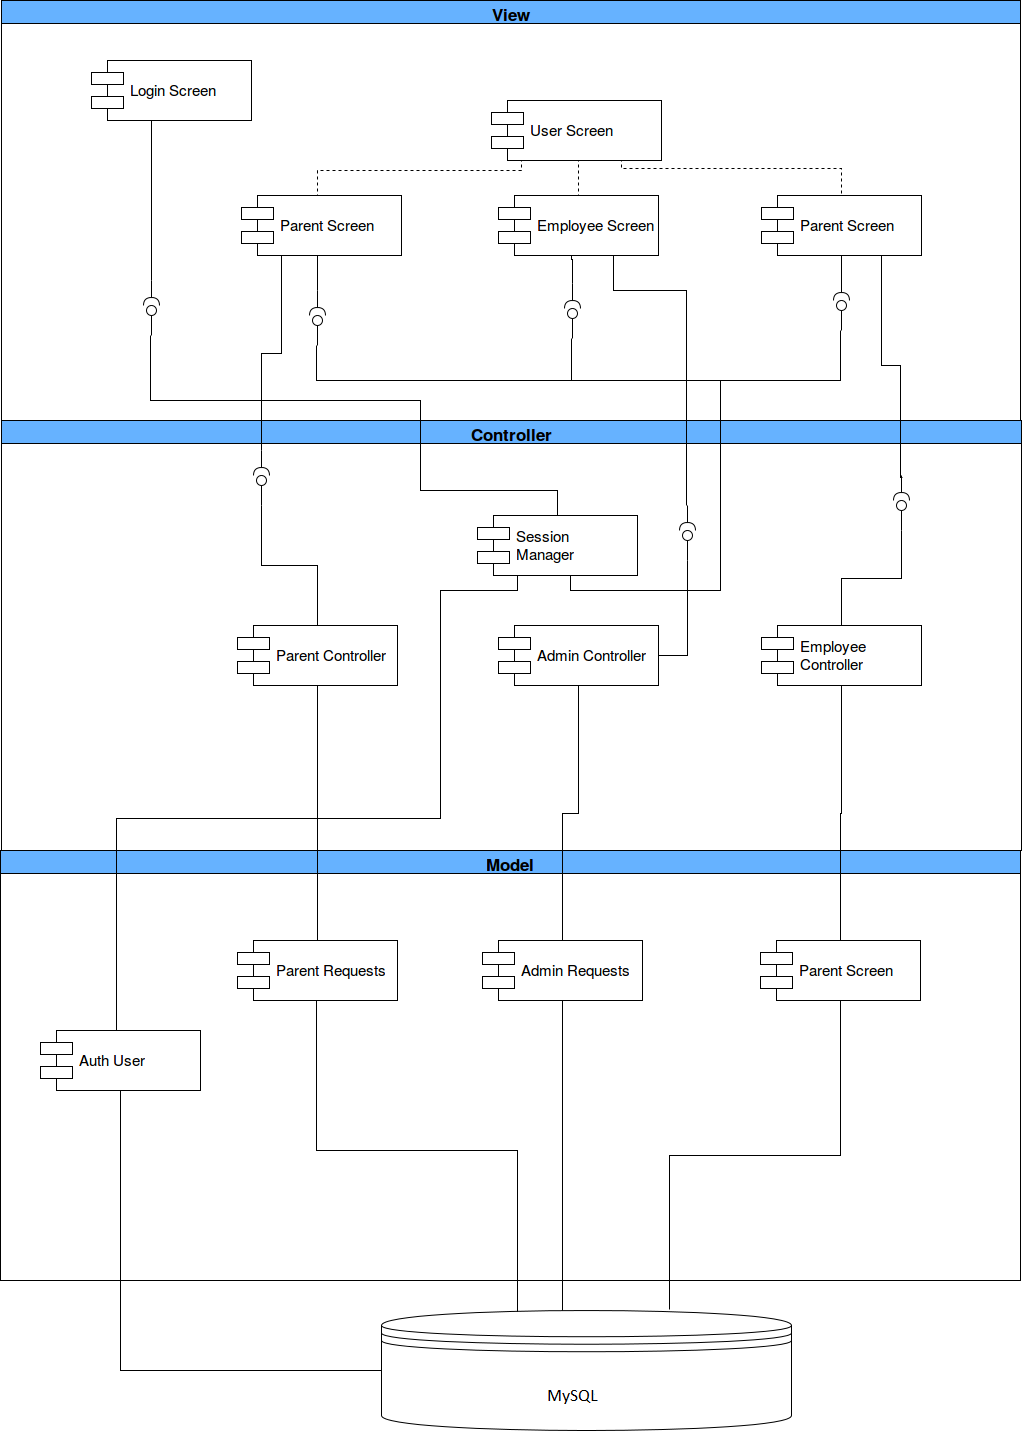
\includegraphics[width=1.08\textwidth]{component/Komponentendiagramm.png}
\end{figure}
\newpage
Wir verwenden Java, Spring Framework, Prime Faces, CSS und H2

\subsection{Spring Framework}
Das Spring Framework ist eine Grundlage für Webbasierte Anwendungen im Stil des MVC Models. Das MVC Model eignet sich gut für diese Anwendung, da verschiedene Teile des Programms unabhänging voneinander bearbeitet und ausgetauscht werden können.

\subsection{Prime Faces/ CSS}
Wir gestalten das Front-End mit Prime Faces und CSS.

\subsection{H2}
H2 dient als Datenbankabbildung.

\subsection{Testen}
Das Testen unserer Anwendung erfolgt mit Selenium für GUI Tests und JUnit für weitere Testfälle.

\subsection{Version Control}
Um das parallele Arbeiten zu erleichtern, verwenden wir Git.


\newpage
\begin{figure}
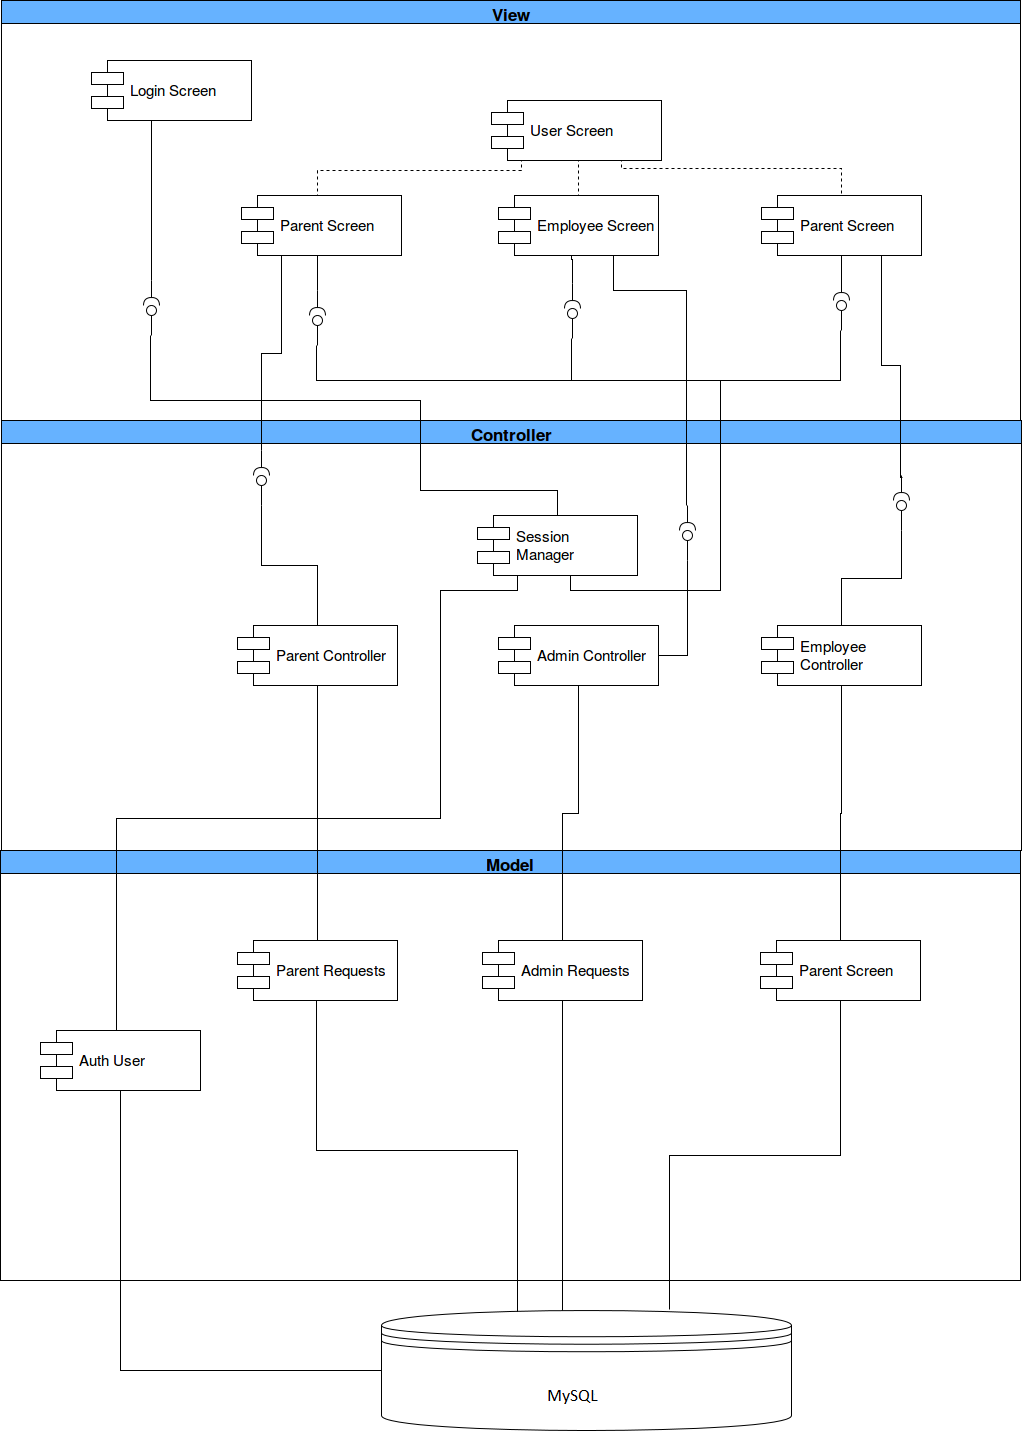
\includegraphics[scale=0.4]{component/Komponentendiagramm.png}
\end{figure}
